%!TEX root = ../thesis.tex
\chapter{Gravitational lensing formalism}
\label{chapter:gravitational-lensing-formalism}

\section{Mathematical preliminaries}

The essence of General Relativity (GR) is very elegantly summarised by John Wheeler \citep[pg.235]{wheeler2000geons} in a sentence: matter tells spacetime how to curve, and spacetime tells matter how to move. 

The first half of this statement is quantified by the Einstein Field Equations (EFEs), which is the analogue of Poisson's equation in Newtonian gravity. They are a group of 10 coupled differential equations that describe the interaction between matter and geometry of spacetime, given by (in tensor notation)

\begin{equation}
  G_{\mu \nu} + \Lambda g_{\mu \nu} = 8\pi T_{\mu \nu}
  \label{eq:efes}
\end{equation}
where $g_{\mu \nu}$ is the metric of spacetime, $\Lambda$ is the cosmological constant, $G_{\mu \nu}$ is the Einstein tensor and $T_{\mu \nu}$ is the energy-momentum tensor. The energy momentum tensor on the right hand side is a source term that encodes how matter is distributed in the universe, and on the left hand side the Einstein tensor depends on the metric tensor, which describes the spacetime geometry. For a perfect pressureless fluid, the energy momentum tensor is

\begin{equation}
  T^{\mu \nu} = \rho u^{\mu} u^{\nu}
\end{equation}
where $u^{\mu}$ is the 4-velocity of the fluid. 

If we solve Einstein's field equations, we can obtain the metric tensor $g_{\mu \nu}$, which encodes the spacetime geometry. The metric tensor then influences how a particle behaves in this spacetime, bringing us to the second part of the statement: spacetime tells matter how to move. Given a metric tensor $g_{\mu \nu}$, we can first write down the line element

\begin{equation}
  ds^2 = g_{\mu \nu} dx^{\mu} dx^{\mu}
  \label{eq:line-element}
\end{equation}

Equations of motion of a particle moving in this spacetime can then be derived by first considering the Lagrangian of this particle

\begin{equation}
  \mathcal{L} = \sqrt{g_{\mu \nu} \frac{dx^{\mu}}{d \lambda} \frac{dx^{\nu}}{d \lambda}}
\end{equation}
where $\lambda$ is an affine parameter which increases monotonically along the particle's worldline and $x^{\mu}(\lambda)$ describes the trajectory of the particle. Between two spacetime points $A$ and $B$, we want to maximize $\int^{A}_{B} L(x^{\mu}, \dot{x}^{\mu})\, d \lambda$, so $\mathcal{L}$ satisfies the Euler-Lagrange (E-L) equations

\begin{equation}
  \frac{\partial \mathcal{L}}{\partial x^{\mu}} - \frac{d}{d \lambda}\left ( \frac{\partial \mathcal{L}}{\partial \dot{x}^{\mu}} \right ) = 0.
  \label{eq:euler-lagrange-eqn}
\end{equation}

From the E-L equations we arrive at the geodesic equation

\begin{equation}
  \ddot{x}^{\mu} + \Gamma^{\mu}_{\alpha \beta} \dot{x}^{\alpha} \dot{x}^{\beta} = 0 
  \label{eq:geodesic-eqn}
\end{equation}
where an overdot represents a derivative with respect to the affine parameter $\lambda$, and $\Gamma$ are the Christoffel symbols given by

\begin{equation}
  \Gamma^{\mu}_{\alpha \beta} = \frac{1}{2} g^{\mu \rho} (g_{\rho \alpha, \beta} + g_{\rho \beta, \alpha} - g_{\alpha \beta, \rho}).
  \label{eq:christoffels}
\end{equation}

A freely moving particle always moves along a geodesic, which is a generalisation of the notion of "straight lines" to a curved spacetime. In addition, light, as a massless particle, travels along null geodesics, in contrast to timelike ones for massive particles. Therefore, all light trajectories have to satisfy the null condition

\begin{equation}
  g_{\mu \nu} dx^{\mu} dx^{\nu} = 0.
  \label{eq:null-condition}
\end{equation}

The result is a handful of coupled differential equations that need to be solved to find the trajectory of light. Nevertheless, a common problem arising in cosmology stems from the fact that as soon as we depart from the simplest homogeneous models used by observational cosmologists, the task of finding solutions to null geodesics quickly becomes an intractable analytical problem. In our work, we instead use a numerical method to integrate the null geodesics to find the trajectory of the photon. 

\section{Derivation of bending angle in the Schwarzschild metric}

It is useful to first revise gravitational lensing in a universe without $\Lambda$, in a Schwarzschild metric, which is well understood. This will form the basis for our comparison with a universe that includes $\Lambda$. 

Spacetime outside a spherically symmetric distribution of matter and vacuum everywhere else is described by the Schwarzschild metric, one of the first known solutions to Einstein's field equations. Its line element is given by

\begin{equation}
  ds^2 = -\left ( 1- \frac{2M}{r} \right ) dt^2 + \left ( 1 - \frac{2M}{r}\right )^{-1} dr^2 + r^2(d\theta^2 + \sin^2\theta d \phi^2).
  \label{eq:schwarzschild-metric}
\end{equation}
where $M$ is the central mass. 

Due to spherical symmetry, we can restrict ourselves to the equatorial plane $\theta = \pi/2$ without loss of generality. This metric is asymptotically flat as $r \rightarrow \infty$. We can then find the total deflection angle $\alpha$ experienced by light that comes in from $r=-\infty$, gets deflected, and travels on towards $r=+\infty$ as 

\begin{equation}
  \alpha = 2 \int_{r_0}^{\infty} \left |  \frac{d\phi}{dr} \right | dr - \pi
\end{equation}
where $r_0$ is the distance of closest approach. 

The static nature and spherical symmetry of the Schwarzschild metric implies that there are two constants of motion for any particle traveling in this geometry. These can be obtained through direct application of the E-L equation (\autoref{eq:euler-lagrange-eqn}), and we have

\begin{subequations}
  \begin{align}
    E &= \left ( 1 - \frac{2M}{r} \right ) \dot{t},\\
    L &= r^2\dot{\phi}.
  \end{align}
  \label{eq:schwarzschild-constants}
\end{subequations}

By applying the null condition (\autoref{eq:null-condition}) on the metric, we obtain an expression for $\frac{d\phi}{dr}$

\begin{equation}
  \frac{d\phi}{dr} = \pm \frac{1}{r^2} \sqrt{\frac{1}{ \frac{1}{b^2} - \left (1- \frac{2M}{r} \right )\frac{1}{r^2} }}
  \label{eq:dphi-dr}
\end{equation}
where $b = L/E$ is the impact parameter (since $\frac{d\phi}{dr} = \dot{\phi}/\dot{r}$). Integrating this (for a detailed derivation see \cite{keeton2005formalism}), we obtain an expression for the bending angle $\alpha$ as a series expansion in $M/r_0$. This series, to third order in $M/r_0$, is as follows:

\begin{equation}
  \alpha = 4 \frac{M}{r_0} + \left ( -4 + \frac{15\pi}{4} \right )\left ( \frac{M}{r_0}\right )^2 + \left ( \frac{122}{3} - \frac{15\pi}{2} \right )\left ( \frac{M}{b}\right )^2.
  \label{eq:lensing-series-expansion-r0}
\end{equation}

This can be easily converted to a series in $M/b$ instead of $M/r_0$, which is usually done in literature, since a relation between $b$ and $r_0$ can be derived in a series expansion by setting $\dot{r} = 0$, giving \citep{keeton2005formalism}

\begin{equation}
  r_0 = b \left [ 1 - \frac{M}{b} - \frac{3}{2} \left ( \frac{M}{b}\right)^2 - 4\left ( \frac{M}{b}\right)^3 \right ].
  \label{eq:b-r0-relation}
\end{equation} 

This relation can then be used to rewrite the expansion in terms of $\frac{M}{b}$ to give us

\begin{equation}
  \alpha = 4 \frac{M}{b} + \frac{15\pi}{4} \left ( \frac{M}{b} \right )^2 + \frac{128}{3} \left ( \frac{M}{b} \right )^3.
  \label{eq:series-expansion-b}
\end{equation}
and indeed many authors use the impact parameter to discuss the bending of light in Schwarzschild spacetime \citep{wald2010general,misner2017gravitation,butcher2016no}. However, it has been pointed out previously by other authors \citep{ishak2008new,hammad2013note,lebedev2013influence} that in the non-zero $\Lambda$ case, the definition of the impact parameter is no longer independent of $\Lambda$ and this definition becomes questionable as spacetime is no longer asymptotically flat. 

In this work we will use another constant of the motion for the non-zero $\Lambda$ case, and for consistency we will use that parameter here as well so that a fair comparison can be made, even though the Schwarzschild case does not include a cosmological constant.

We can define another constant of the motion $R_u$ which corresponds to the unperturbed trajectory of light (see \autoref{fig:lensing}), which is related to $r_0$ by (see Eq. 6 of \citet{ishak2008new} and Eq. 3 of \citet{butcher2016no}).

\begin{equation}
  \frac{1}{r_0} = \frac{1}{R_u} + \frac{M}{R_u^2} + \frac{3M^2}{16R_u^3}
  \label{eq:r0-R-relation}
\end{equation}
where I have added a subscript $u$ to differentiate it from the Kottler coordinate $R$ in the next chapter. Using this relation and applying it to \autoref{eq:lensing-series-expansion-r0}, we can get a series expansion in $M/R_u$, which, up to third order, is given by

\begin{equation}
  \alpha = 4 \frac{M}{R_u} + \frac{15\pi}{4} \left ( \frac{M}{R_u} \right )^2 + \frac{401}{12} \left ( \frac{M}{R_u} \right )^3.
  \label{eq:series-expansion-R}
\end{equation}

There are 3 length quantities that are typically used in Schwarzschild lensing: the distance of closest approach $r_0$, the impact parameter $b$, and the parameter of the unperturbed trajectory $R_u$. They are related to each other through \autoref{eq:b-r0-relation} and \autoref{eq:r0-R-relation}, and their related series expansions are respectively given by \autoref{eq:lensing-series-expansion-r0}, \autoref{eq:series-expansion-b} and \autoref{eq:series-expansion-R}. The coefficient of the leading order term is the same for all three but they differ on higher order terms in the series expansion. Many gravitational lensing anayses done on the Schwarzschild metric are only concerned with the leading order term, and hence use these three lengths somewhat interchangeably. But in this project we are interested in corrections at the second order or higher, and the distinction becomes important. In the subsequent section of the report, we will be using the series expansion in $M/R_u$ (\autoref{eq:series-expansion-R}). 

As mentioned previously, \citet{rindler2007contribution} proposed a different expression for $\alpha$. The expression was later refined for a Swiss-cheese universe \citep{ishak2008new}, and I will state it here (in our notation) for easy comparison:

\begin{equation}
  \alpha_{\text{Ishak}} = 4 \frac{M}{R_u} + \frac{15\pi}{4} \left ( \frac{M}{R_u} \right )^2 + \frac{305}{12} \left ( \frac{M}{R_u} \right )^3 - \frac{\Lambda R_u R_h}{3},
  \label{eq:rindler-ishak-alpha}
\end{equation}
where $R_h$ is the boundary of the hole in static coordinates in the Swiss-cheese model. The $\Lambda$-term is negative, and they postulate that the cosmological constant attenuates lensing. 

\section{Lensing observables}

A significant part of the conflict in literature comes from the question of which quantities in lensing are observable, and whether these observable quantities are ultimately affected by the presence of the cosmological constant. Therefore we aim to stick with strictly observable quantities. 

\begin{figure}
  \centering
  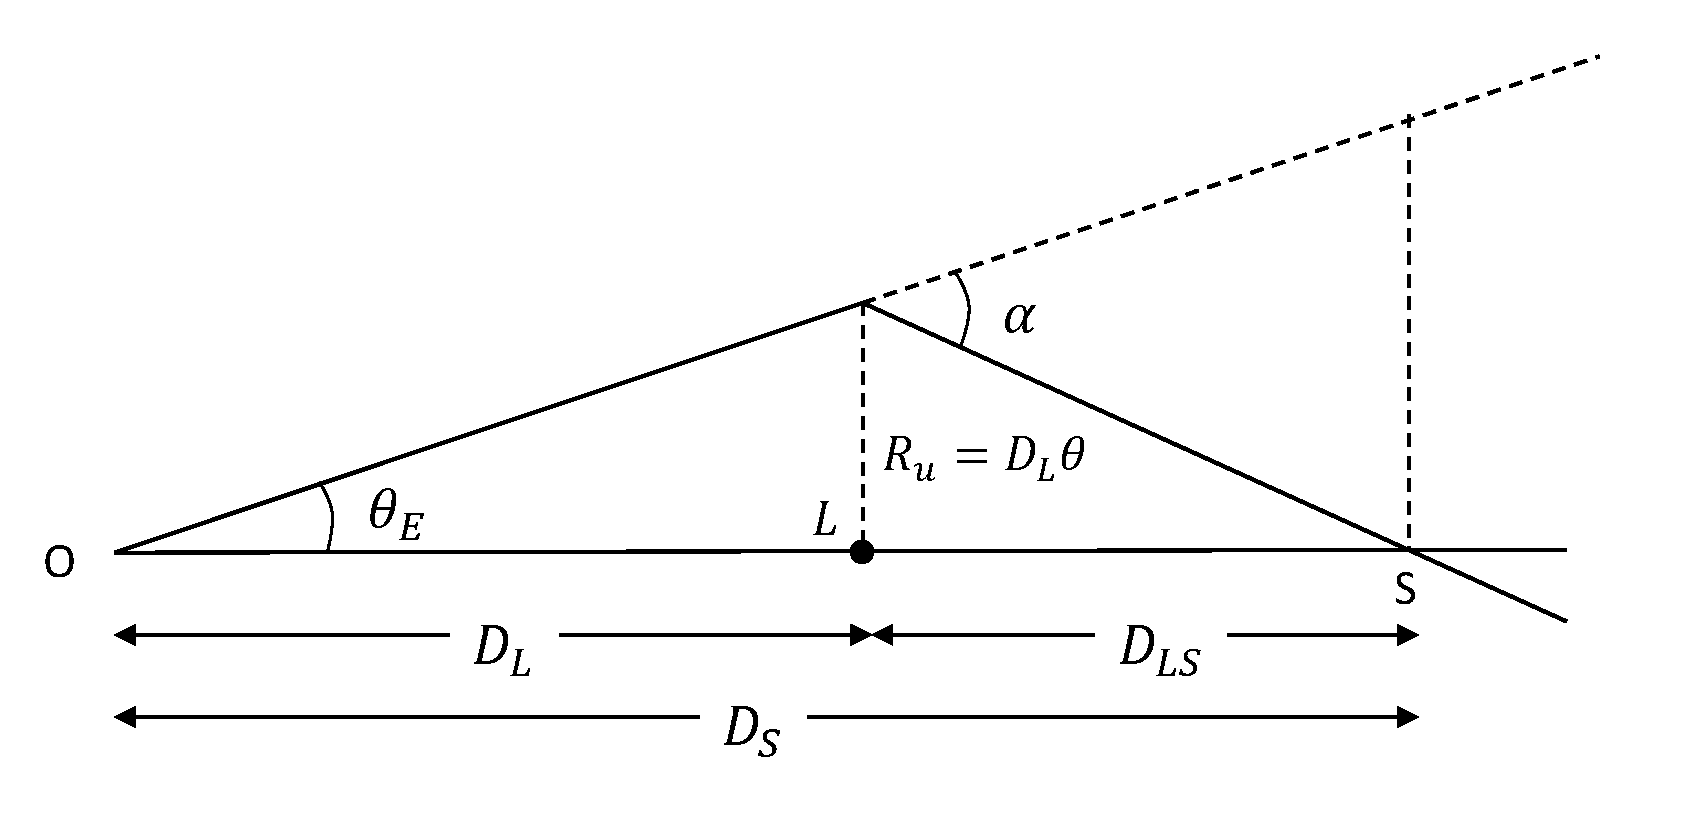
\includegraphics[height=0.4\linewidth]{images/lensing_cropped.pdf}
  \caption{Diagram of gravitational lensing, where the lens, observer, and source are collinear.}
  \label{fig:lensing}
\end{figure}

We consider a simple picture where the observer, lens, and source are aligned, as shown in \autoref{fig:lensing}. Bending is assumed to happen at a single point above the lens, since the distance from the observer to the lens and source is assumed to be much larger than the distance of closest approach between the light ray and the lens. From this diagram we can easily, with some trigonometry, obtain the lens equation \citep{schneider1992gravitationallenses}

\begin{equation}
  D_S \theta_E = D_{LS} \alpha
  \label{eq:lens-eqn}
\end{equation}
where $\alpha$ is the bending angle as previously derived, $D_S$ is the angular diameter distance from observer to source, $D_{LS}$ is the angular diameter distance from lens to source, and $\theta_E$ is known as the Einstein angle. $R_u$ can also be expressed in terms of the observable quantities $R_u = D_L \theta_E$, where $D_L$ is the angular diameter distance from observer to the lens.  

With this in mind, we can begin looking at the Swiss-cheese model, and look to apply this formalism in such a universe. 